\chapter{原子核的衰变}
不稳定核在嬗变成(更)稳定原子核的过程中,会发生$\alpha$衰变、$\beta$衰变、$\gamma$跃迁、中子发射、质子发射或自发裂变等过程。

\section{\textalpha 衰变}

$\alpha$衰变的形式:
\begin{align}
	{^A_Z\nuc X} \to {^{A-4}_{Z-2}\nuc Y} + {^4_2\nuc{He}}.
\end{align}
%子核较母核减少了2个质子和2个中子。
%由于$\beta$稳定曲线偏向$N$轴,位于$\beta$稳定曲线上的母核发生$\alpha$衰变后,子核会偏离$\beta$稳定曲线,故子核可能会接着发生$\beta$衰变。
$\alpha$衰变的特点:
\begin{compactenum}
	\item 重核$A>140$;
	\item 能量既不太大也不太小$\SIrange{4}{9}{MeV}$;
	\item 半衰期范围较大$\SI{e-7}{s}\vs\SI{e15}{yr}$。
\end{compactenum}
由液滴模型,$\alpha$衰变主要项是Coulomb排斥。

自发的衰变需要释放能量,由比结合能曲线:不存在发射$\nucli2H$核的衰变,重核发生$\alpha$衰变将释放能量,子核也比母核更稳定。\footnote{事实上释放$\nucli{12}C$等粒子的衰变释放能量更多,子核更稳定,但是其发生概率太小。}

\subsection{\textalpha 衰变能}

对于静止\footnote{母核热运动的动能$\ll\alpha$衰变的衰变能。}的母核,衰变前后有能量守恒
\[
	m_{\nuc X}c^2=m_{\nuc Y}c^2+m_\alpha c^2+T_{\nuc Y}+T_\alpha
\]
$\alpha$衰变能就等于子核$\nuc Y$和$\alpha$粒子的动能之和,即衰变前后静止质量之差
\begin{align}
	E_0&=T_{\nuc Y}+T_\alpha=\bigfkh{m_{\nuc X}-(m_{\nuc Y}+m_\alpha)}c^2\\\notag
	&=\D(\nuc X)-\D(\nuc Y)-\D(\alpha)
\end{align}
故$\alpha$衰变的必要条件为$E_0>0$
\[
	M(\nuc X)>M(\nuc Y)+M(\alpha)
\]

由液滴模型的Coulomb能:$A,Z$越大,$\alpha$衰变能越大;但是对于同位素$A$越大,$\alpha$衰变能越小。

壳层结构给出:母核$N=126$时,$\alpha$衰变能很小;子核$N=126$时,$\alpha$衰变能局部极大。

\paragraph{$\alpha$衰变能与核能级图}
由静止母核发生$\alpha$衰变前后的能量、动量守恒推出
\begin{align}
	E_0=\frac{A}{A-4}T_\alpha
\end{align}
故可以通过测量$\alpha$粒子的能量$T_\alpha$得到$\alpha$衰变能$E_0$。\footnote{Y的轨迹$\ll\alpha$粒子,难以测量其能量。}

然而,单一能级衰变的母核可能衰变出不同能级的子核,导致$\alpha$粒子有多个能量。衰变能之间的差对应子核的能级结构。
其中,最大衰变能很有可能就是子核的基态。
\iffalse
基态-基态的$\alpha$衰变能为
\begin{align}
	E_0=M(\nuc X)-M(\nuc Y)-M(\alpha),
\end{align}
式中皆为基态质量。
\fi
\begin{center}
	\includegraphics[page=4]{figures/tikz/layouts.pdf}
	\captionof{figure}{$\alpha$衰变的衰变纲图}
\end{center}

\subsection{\textalpha 衰变的衰变常数}

$\alpha$粒子在核内主要受核力和Coulomb力。其中核内所受合力平衡,所以$\alpha$粒子在核内自由地高速运动。

隧穿理论:$\alpha$粒子相对于子核的势能
\begin{align}
	V(r)=\begin{cases}
		-V_0,&r<R\\
		\frac1{4\pi\varepsilon_0}\frac{2Z_{\nuc Y}e^2}r,&r\geqslant R
	\end{cases}
\end{align}
其中$R=R_\alpha+R_{\nuc Y}$。
\begin{center}
	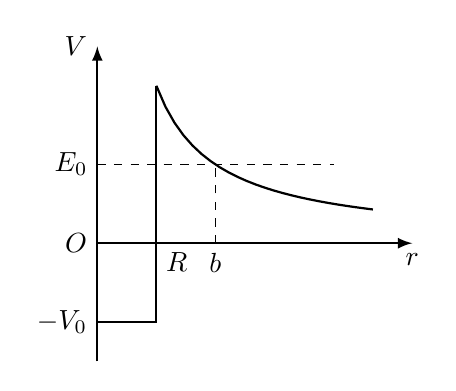
\begin{tikzpicture}
		\draw[thick, -latex](0, -1.5)--(0, 2.5)node[left]{$V$};
		\draw[thick, -latex](0, 0)node[left]{$O$}--(4, 0)node[below]{$r$};
		\draw[dashed](0, 1)node[left]{$E_0$}--(3, 1);
		\draw[thick](0, -1)node[left]{$-V_0$}--(.75, -1)--(.75, 2);
		\draw[dashed](1.5, 0)node[below]{$b$}--(1.5, 1);
		\node[below right]at(.75, 0){$R$};
		\draw[thick, domain=.75:3.5]plot(\x, {1.5/\x});
	\end{tikzpicture}
	\captionof{figure}{Coulomb势垒}
\end{center}
量子力学中我们学过,能量为$E$质量为$m$的粒子穿过高度为$V_0$宽度为$a$的方势垒的概率为
\[
	P=\exp\fkh{-\frac{2a}\hbar\sqrt{2m(V_0-E)}},
\]
若衰变发生,$\alpha$粒子需要穿过Coulomb势垒
\[
	P=\exp\fkh{-2\frac{\sqrt{2\mu}}\hbar\int_R^b\sqrt{V(r)-E_0}\d r}=:\e{-G},
\]
式中$\mu=\frac{m_\alpha m_{\nuc Y}}{m_\alpha+m_{\nuc Y}},b=\frac{2Z_\nuc Ye^2}{4\pi\varepsilon_0 E_0}$其中$G$为Gamow因子。对于$b\gg R$有
\[
	P=\e{-G}=\exp\fkh{-\frac{e^2\sqrt{2m_\alpha}}{2\varepsilon_0\hbar}\cdot\frac{Z_\nuc Y}{\sqrt{E_0}}+\frac{4e\sqrt{m_\alpha }}{\sqrt{\pi\varepsilon_0\hbar}}\sqrt{RZ_\nuc Y}}
\]
这个概率乘上$\alpha$粒子到达边界的频率
\[
	n=\frac{\nu}{2R}\doteq\frac1{2R}\sqrt{\frac{2(E_0+V_0)}{m_\alpha}}\doteq\SI{2.44e21}{/s}.
\]
就得到了衰变常数$\lambda=nP$。
\begin{align}
	\lg\lambda=C-1.72\times Z_{\nuc Y}E_0^{-1/2}
\end{align}
式中$C$是影响较小的其他项。

对于奇$A$核和奇奇核,理论与实验差别较大:引入阻碍因子(Hindrance factor):
\begin{compactenum}
	\item 形成因子:$\alpha$粒子并非早已存在,是在衰变过中产生的;
	\item 角动量:会产生离心势$\frac{\ell(\ell+1)\hbar^2}{2m_\alpha R^2}.$
\end{compactenum}
\paragraph{总结}
\begin{compactenum}
	\item $\alpha$粒子穿透势垒的概率$P$是决定衰变常数$\lambda$的最主要因素;衰变能$E_0$越大,所需要穿透的势垒越薄,$\lambda$越大,衰变得越快。
	\item $\alpha$粒子还可能带走角动量,离心势会加高势垒,减小了衰变常数。
\end{compactenum}
让衰变能大一些,让$\alpha$粒子带的角动量小一点,有利于$\alpha$衰变的发生。

\subsection{\textalpha 衰变的宇称和角动量}

$\alpha$衰变过程中角动量守恒,若母子核的角动量分别为$I_\ini,I_\fin$,则$\alpha$粒子的角动量$\ell_\alpha$可取
\begin{align}
	\ell_\alpha=|I_\ini-I_\fin|,\ldots,I_\ini+I_\fin
\end{align}
共$2\min\{I_\ini,I_\fin\}+1$种情况。

在强相互作用和电磁相互作用中,宇称是守恒的。$\alpha$粒子的宇称$(-)^{\ell_\alpha}$,因此初末态宇称若不满足
\begin{align}
	\pi_\ini=\pi_\fin\cdot(-)^{\ell_\alpha},
\end{align}
则$\alpha$衰变不可能发生!

\section{\textbeta 衰变}

原子核自发地放出$\beta$粒子或俘获轨道电子,并转变成另一种原子核的现
象,称为$\beta$衰变,有三种形式:
\begin{compactenum}
	\item $\beta^-$衰变:原子核衰变时发射负电子;
	\item $\beta^+$衰变:原子核衰变时发射正电子;
	\item 轨道电子俘获(orbital electron capture, EC,也称$\varepsilon$衰变):原子核从核外的电子壳层俘获一个轨
	道电子。
\end{compactenum}

由于质子中子之间质量存在差异
\[
	m_\nton - m_\pton = \SI{1.293}{\MeV}/c^2 > m_\elc = \SI{0.511}{MeV}/c^2
\]
故自由中子可以发生$\beta^-$衰变:
\[
	\nton\to\pton+\elc^-\textcolor{lightgray}{\,+\,\bar\nu_\elc},
\]
而自由质子(即$\nucli1H$)不能发生$\beta^+$衰变和EC:
\begin{gather*}
	\pton\nrightarrow \nton+\elc^+\textcolor{lightgray}{\,+\,\nu_\elc},\\
	\pton+\elc^-\nrightarrow \nton\textcolor{lightgray}{\,+\,\nu_\elc},
\end{gather*}
只有结合在核中的质子才行。

\paragraph{$\beta$衰变的特点}
\begin{compactenum}
	\item $\beta$衰变核素遍及整个元素周期表;
	\item $\beta$衰变不改变$A$,子母核同属等量异位素;
	\item $\beta$衰变电子能谱分布是连续的:$\si{keV}\vs\si{MeV};$
	\item 半衰期范围$10^{-3}\,\mathrm{s}\vs\SI{e24}{yr}.$
\end{compactenum}
由于$\beta$衰变不改变$A$,考虑液滴模型\eqref{liquid-drop model BE}中与$Z$有关的项
\[
	B=\textcolor{lightgray}{a_VA-a_SA^{2/3}}-a_\mathrm C\frac{Z^2}{A^{1/3}}-a_\mathrm{sym}\frac{(A/2-Z)^2}{A}+a_\mathrm p\frac{\delta}{A^{1/2}},
\]
得出质量
\[
	M(Z,A)=\textcolor{lightgray}{Am_\nton\,+\,}Z\bigkh{M(\nucli1H)-m_\nton}+B,
\]
Coulomb能、对称能使得等量异位素的结合能是一条抛物线,%而最稳定的核素约处于$Z=A/2$的位置,
小$Z$会发生$\beta^-$衰变,大$Z$会发生$\beta^+$衰变或EC;对于偶$A$核,由于对能项,奇奇核与偶偶核会有各自的抛物线。

\paragraph{$\beta$-ray's wrong energy}子核能级分立,但$\beta$粒子的能量是连续的?
\begin{compactitem}
	\item 假说1:子核能级密集$\nleftarrow$~$\gamma$能谱不连续;
	\item 假说2:$\beta$粒子与介质作用损失了不等的能量$\nleftarrow$厚壁量热器实验。
\end{compactitem}
Pauli中微子假说(1930):原子核在$\beta$衰变的过程中,不仅放出一个$\beta$粒子,同时还放出一个中性微小粒子。
\paragraph{中微子假说}中微子性质:
\begin{compactenum}
	\item 电荷为0;
	\item 自旋为$\hbar/2$,是Fermi子;
	\item 质量非常小,\href{https://www.sciencedirect.com/topics/chemistry/electron-neutrino}{$<\SI{0.07}{eV}/c^2$},\footnote{中微子震荡(\nobel{2015})表明中微子质量不严格是0。}与电子相比,可以看作0;
	\item 磁矩非常小,\href{https://arxiv.org/ftp/arxiv/papers/1506/1506.01284.pdf}{$\sim 10^{-19}\muB$};
	\item 与物质的相互作用非常弱,属弱相互作用。
\end{compactenum}
$\nu$和$\bar\nu$互为反粒子,$\nu$左旋,$\bar\nu$右旋。相互作用性质不同。

\subsection{\textbeta 衰变的三种类型}

$\beta^-,\beta^+,$EC:
\begin{align}
	\beta^-:&\qquad{^A_Z\nuc X} \to {^{\quad\!A}_{Z+1}\nuc Y} + \elc^- + \bar\nu_\elc,\\
	\beta^+:&\qquad{^A_Z\nuc X} \to {^{\quad\!A}_{Z-1}\nuc Y} + \elc^+ + \nu_\elc,\\
	\mathrm{EC}:&\qquad{^A_Z\nuc X} + \elc^- \to {^{\quad\!A}_{Z-1}\nuc Y} + \nu_\elc
\end{align}
丰中子核素大多具有$\beta^-$衰变,比如天然放射系、重核裂变、$(n,\gamma)$反应后的核素;丰质子核素可以发生$\beta^+$衰变或EC,比如$(\gamma,n)$反应后的核素。

定义:$\beta^-$衰变放出的动能$T_{\nuc Y}+T_{\beta^-}+T_{\bar\nu_\elc}$为$\beta^-$衰变能。
\begin{align}\notag
	E_0(\beta^-)&=[m(\nuc X)-m(\nuc Y)-m_\elc]c^2\\\notag
	&\doteq[M(\nuc X)-\cancel{Zm_\elc}-M(\nuc Y)+\cancel{(Z+1)m_\elc}-\cancel{m_\elc}]c^2\\
	&=[M(\nuc X)-M(\nuc Y)]c^2\\\notag
	&=\D(Z,A)-\D(Z+1,A);
\end{align}
$\beta^+$和EC衰变能定义类似:
\begin{align}
	E_0(\beta^+)&=[M(\nuc X)-M(\nuc Y)-2m_\elc]c^2;\\
	E_0(\varepsilon)&=[M(\nuc X)-M(\nuc Y)]c^2-\varepsilon_i.
\end{align}
其中,$\varepsilon_i(i=\mathrm{K,L,M,}\ldots)$为被俘获电子与母核的结合能,
\begin{align*}
	\varepsilon_{\mathrm K}&\doteq(Z-1)^2\,\si{Ry},\\
	\varepsilon_{\mathrm L}&\doteq\frac14(Z-5)^2\,\si{Ry},\\\
	\varepsilon_{\mathrm M}&\doteq\frac19(Z-13)^2\,\si{Ry}.
\end{align*}
其中$\si{Ry}$是Rydberg能量单位,$\SI{1}{Ry}=\SI{13.6}{eV}$。

一般都是K层电子最容易发生俘获,但当衰变能不高时,就会发生L层俘获,满足
\[
	\varepsilon_\mathrm K / c^2 > M(\nuc X)-M(\nuc Y) > \varepsilon_\mathrm L / c^2
\]

当EC发生时,原子会发射特征X射线以及Auger电子。比如当K层电子被俘获时,子核的L层电子就会向K层跃迁,产生能量为$\varepsilon_\mathrm K - \varepsilon_\mathrm L$的X射线;该能量也可以直接给予L层的电子使其电离,产生能量为$\varepsilon_\mathrm K - 2\varepsilon_{\mathrm L}$的Auger电子。

由于衰变能限制,因此发生$\beta$衰变的能量条件为:
\begin{align}
	\beta^-:&\qquad M(\nuc X)>M(\nuc Y)\\
	\beta^+:&\qquad M(\nuc X)-M(\nuc Y) > 2m_\elc,\\
	\mathrm{EC}:&\qquad M(\nuc X)-M(\nuc Y) > \varepsilon_i / c^2.
\end{align}
由于
\[
	2m_\elc c^2=\SI{1.022}{MeV}\gg\varepsilon_i,
\]
故若可以发生$\beta^+$衰变,则一定也可以发生EC。对于衰变能较大的轻核,$\beta^+$衰变概率显著,重核反之,中等质量核二者几率相仿。一些核(如$\nucli{64}{Cu}$)可能同时满足三个条件,可以同时以三种方式进行衰变。
\begin{center}
	\includegraphics[page=6]{figures/tikz/layouts.pdf}
	\captionof{figure}{$\nucli{64}{Cu}$的衰变纲图}
\end{center}

\subsection{\textbeta 衰变的Fermi理论和选择定则}

$\beta$粒子从何而来?
\begin{compactenum}
	\item 质子和中子是核子两种不同的量子态,$\beta$衰变是核中质子和中子两种量子态之间的跃迁;
	\item 核子两种量子态跃迁过程中放出电子和中微子,它们是核子不同状态跃迁的产物;
	\item $\beta$衰变中放出电子和中微子,电子-中微子场与原子核的相互作用为弱相互作用,半衰期($\SI{e-3}{s}\vs\SI{e18}{yr}$)比电磁相互作用($\SIrange{e-16}{e-4}{s}$)要长得多。
\end{compactenum}
Fermi黄金规则
\begin{align}
	\lambda = \frac{2\pi}\hbar\abs{V_{\fin\ini}}^2\rho(E_\fin),
\end{align}
式中$V_{\fin\ini}$是跃迁矩阵元,$\rho(E_\fin)$是末态密度。

量子力学的微扰理论给出:单位时间发射动量处于$(p,p+\d p)$间的$\beta$粒子的概率为:
\[
	I(p_\beta)\d p_\beta=\frac{2\pi}\hbar\abs{\int\psi_\fin\cj H\psi_\ini\d^3r}^2\dv n{T_\beta}
\]
初态$\psi_\ini=u_\ini$母核波函数,末态$\psi_\fin=u_\fin\varphi_\beta\varphi_\nu$子核、$\beta$和中微子波函数,$H=g$描述弱作用强度:
\[
	I(p_\beta)\d p_\beta=\frac{2\pi g^2}\hbar\abs{\int u_\fin\cj\varphi_\beta\cj\varphi_\nu\cj u_\ini\d^3r}^2\dv n{T_\beta}
\]

原子核对电子和中微子的波场影响很小,可视电子(近似)和中微子为自由粒子,波函数用平面波描述
\[
	\varphi_\beta\cj=V^{-1/2}\e{-\i\bm k_\beta\cdot\bm r},\quad\varphi_\nu\cj=V^{-1/2}\e{-\i\bm k_\nu\cdot\bm r}
\]
则上式化作
\[
	I(p_\beta)\d p_\beta=\frac{2\pi g^2}{\hbar V^2}\abs{M_{\ini\fin}}^2\dv n{T_\beta}
\]
其中跃迁矩阵元
\begin{align}\label{transition matrix element}
	M_{\ini\fin}=\int u_\fin\cj u_\ini\e{-\i(\bm k_\beta+\bm k_\nu)\cdot\bm r}\d^3r
\end{align}

\paragraph{末态密度}$\beta$和中微子状态数
\[
	\d n_\beta=\frac V{h^3}4\pi p_\beta^2\d p_\beta,\quad \d n_\nu=\frac V{h^3}4\pi p_\nu^2\d p_\nu
\]
故末态密度
\[
	\dv n{T_\beta}=\frac{p_\beta^2p_\nu^2\d p_\beta\nd p_\nu}{4\pi^4\hbar^6\d T_\beta}V^2
\]
忽略子核反冲动能\footnote{因为子核质量$\gg$轻子。},则:
\[
	T_\nu+T_\beta=E_0
\]
考虑到$m_\nu=0,T_\nu=cp_\nu$
\[
	p_\nu=\frac{E_0-T_\beta}c,\quad\dv{p_\nu}{T_\beta}=-\frac1c.
\]
带入上式
\[
	\dv n{T_\beta}=\frac{p_\beta^2(E_0-T_\beta)^2\d p_\beta}{4\pi^4\hbar^6c^3}V^2
\]
故$m_\nu=0$时的$\beta$跃迁几率公式
\begin{align}\label{beta-decay Prob}
	I(p_\beta)\d p_\beta=\frac{g^2\abs{M_{\ini\fin}}^2}{2\pi^3\hbar^7c^3}\kh{E_0-\sqrt{p_\beta^2c^2+m_\elc^2c^4}+m_\elc c^2}^2p_\beta^2\d p_\beta
\end{align}
\begin{center}
	\includegraphics[page=7]{figures/tikz/layouts.pdf}
	\captionof{figure}{末态密度$I(p_\beta)$随$\beta$粒子动量$p_\beta$的关系}
\end{center}
若$p_\beta$很小,则
\[
	I(p_\beta)\doteq\frac{g^2\abs{M_{\ini\fin}}^2}{2\pi^3\hbar^7c^3}E_0^2p_\beta^2\propto p_\beta^2;
\]
若$p_\beta$与最大值$p_{\beta\max{}}$相差$\D p_\beta$很小,则
\[
	I(p_\beta)\doteq\frac{g^2\abs{M_{\ini\fin}}^2}{2\pi^3\hbar^7c^3}\kh{\frac{p_{\beta\max{}}^2c^2}{E_0+m_\elc c^2}}^2\D p_\beta^2\propto\D p_\beta^2.
\]
因此$\beta$谱在两端会呈现两个抛物线。

末态密度项决定了$\beta$粒子的动量谱的形状,会影响衰变速度。

事实上,$\beta$粒子还受核Coulomb场的影响,式\eqref{beta-decay Prob}还应加上Coulomb修正因子(Fermi function)
\begin{align}\label{Fermi funtion}
	I(p_\beta)\d p_\beta=\frac{g^2\abs{M_{\ini\fin}}^2}{2\pi^3\hbar^7c^3}F(Z,T_\beta)(E_0-T_\beta)^2p_\beta^2\d p_\beta
\end{align}
当$Z$较小时,用非相对论近似
\[
	F(Z,T_\beta)=\frac x{1-\e{-x}},\qquad x=\pm\frac{2\pi\alpha Zc}{v_\beta},\quad\text{for}~\beta^\mp.
\]
\paragraph{跃迁矩阵元}在相同动能的情况下,由
\[
	\Ek+mc^2=\sqrt{p^2c^2+m^2c^4},\implies p=\frac1c\sqrt{\Ek^2+2\Ek mc^2},
\]
知,电子带走的动量/角动量更多。

对式\eqref{transition matrix element}跃迁矩阵元中的轻子项做Taylor展开
\begin{align*}
	\exp\fkh{-\frac\i\hbar(\bm p_\beta+\bm p_\nu)\cdot\bm r}=\sum_{\ell=0}^\infty\frac{(-\i)^\ell}{\ell!}\fkh{\frac{(\bm p_\beta+\bm p_\nu)\cdot\bm r}\hbar}^\ell.
\end{align*}
以衰变能$E_0=\SI{1}{MeV}$估计,当电子获得全部衰变能时,轻子组的动量最大,因此有
\[
	\abs{\frac{(\bm p_\beta+\bm p_\nu)\cdot\bm r}\hbar}\leqslant\frac{E_0r}{\hbar c}=\frac{\SI{1}{MeV}\cdot\SI{1.2}{fm}}{\SI{197.4}{MeV.fm}}A^{1/3}<0.05.
\]
故在级数中,第一项贡献最大,以后各项依次很快递减。

或将平面波按不同的轨道角动量$\ell$正交分解为球面波
\[
	\e{-\i(\bm k_\beta+\bm k_\nu)\cdot\bm r}=\sum_{\ell=0}^\infty(2\ell+1)(-\i)^\ell j_\ell\bigkh{(\bm k_\beta+\bm k_\nu)\cdot\bm r}P_\ell(\cos\theta)
\]
球Bessel函数在$kr\ll 1$下的近似为
\[
	j_\ell(kr)\doteq\frac{(kr)^\ell}{(2\ell+1)!}.
\]
Legendre多项式的内积
\[
	\int P_\ell(\cos\theta)P_{\ell'}(\cos\theta)\sin\theta\d\theta\nd\phi=\frac{4\pi}{2\ell+1}\vd_{\ell\ell'}.
\]
故$\ell=0,1,2,\ldots$各项出现的概率
\begin{center}
	\begin{tabular}{cccccc}
		\toprule
		$\ell$&0&1&2&3&$\cdots$\\
		\midrule
		&1&$\frac{(kr)^2}3$&$\frac{(kr)^4}{45}$&$\frac{(kr)^6}{1575}$&$\cdots$\\
		\bottomrule
	\end{tabular}
\end{center}
第1项贡献最大,以后各项依次很快递减,若$\ell=0$被允许有贡献,此时的跃迁被称为\textbf{允许跃迁},对应的矩阵元称为原子核矩阵元$M$,与轻子无关。

允许跃迁有大的衰变常数,但当其被禁戒而贡献为0时,就要考虑禁戒跃迁。$\ell=n\hbar$称为$n$级禁戒跃迁。每级相差$10^{-4}.$
\paragraph{选择定则}在$\beta$衰变的孤立系统中角动量守恒,母子核的角动量差由两个轻子的自旋和轨道角动量决定。
\[
	\bm I_\ini=\bm I_\fin+\bm\ell+\bm s.
\]

\subparagraph{允许跃迁}
$\ell=0$。电子和中微子自旋均为$1/2$,这时$s$只有0和1两种取值:
\begin{compactenum}
	\item 若$s=0$,电子和中微子自旋反平行,单态,
	\[
		\D I=I_\ini-I_\fin=0,
	\]
	称为Fermi选择定则,F跃迁,F相互作用;
	\item 若$s=1$,电子和中微子自旋平行,三重态,
	\[
		\D I=0,\pm 1,
	\]
	称为Gamow-Teller选择定则,G-T跃迁,G-T相互作用。
\end{compactenum}
允许跃迁的宇称选择定则
\[
	\D\pi=(-)^0=+.
\]
\subparagraph{一级禁戒跃迁}
$\ell=1$,则$\abs{\ell+s}=0,1,2$,故一级禁戒跃迁的自旋和宇称选择定则为
\[
	\D I=0,\pm 1,\pm 2,\quad\D\pi=-.
\]
\subparagraph{二级禁戒跃迁}
按理说,自旋选择定则$\D I=0,\pm 1,\pm 2,\pm 3$,但实际为$\D I=\pm 2,\pm 3$,因为低级的跃迁竞争更强。宇称选择定则$\D\pi=+.$
\begin{center}
	\captionof{table}{$\beta$衰变自旋和宇称的选择定则}
	\begin{tabular}{cccc}
		\toprule
		跃迁类型&$\ell$&$\D I$&$\D\pi$\\
		\midrule
		允许跃迁&0&$0,\pm 1$&$+$\\
		一级禁戒跃迁&1&$0,\pm 1,\pm 2$&$-$\\
		二级禁戒跃迁&2&$\pm 2,\pm 3$&$+$\\
		$\cdots$&$\cdots$&$\cdots$&$\cdots$\\
		$n$级禁戒跃迁&$n$&$\pm n,\pm(n+1)$&$(-)^n$\\
		\bottomrule
	\end{tabular}
\end{center}

\subsection{\textbeta 能谱形状与Kurie描绘}

为验证Fermi理论,将式\eqref{Fermi funtion}改写为
\[
	\fkh{\frac{I(p_\beta)}{F(Z,T_\beta)p_\beta^2}}^{1/2}=\frac{g\abs{M_{\ini\fin}}}{\sqrt{2\pi^3\hbar^7c^3}}(E_0-T_\beta)\propto(E_0-T_\beta).
\]
画在坐标图上是一条直线,这就是Kurie图\footnote{Kurie Plot,是Franz N. D. Kurie提出的,中文翻译为库里厄图或居里描绘,跟居里夫妇(Curie)没关系。}

允许跃迁的Kurie图中,由于源的自吸收和散射,在低能区会偏离直线,但高能区线性很好,且与横轴的交点就是衰变能$E_0.$

禁戒跃迁的$M_{\ini\fin}\neq M$与$p_\beta,p_\nu$有关,Kurie图不再是直线,需要加上形状因子(shape factor)修正为直线。
\paragraph{总结}决定$\beta$能谱形状由式\eqref{Fermi funtion}决定,共三个因子:
\begin{compactenum}
	\item 统计因子$(E_0-T_\beta)^2p_\beta^2\d p_\beta$,反映了末态密度数,电子动量分布在两端都是抛物线;
	\item Coulomb修正因子$F(Z,T_\beta)$;
	\item 跃迁矩阵元$\frac{g^2\abs{M_{\ini\fin}}^2}{2\pi^3\hbar^7c^3}.$
\end{compactenum}

\subsection{衰变常数与比较半衰期}

衰变常数
\begin{align*}
	\lambda&=\int_0^{p_{\beta\max{}}}\frac{g^2\abs{M_{\ini\fin}}^2}{2\pi^3\hbar^7c^3}F(Z,T_\beta)(E_0-T_\beta)^2p_\beta^2\d p_\beta
\end{align*}
暂不考虑矩阵元$M_{\ini\fin}$与能量$T_\beta$的关系,定义Fermi积分
\begin{align}
	f(Z,E_0):=\int_0^{p_{\beta\max{}}}F(Z,T_\beta)\kh{\frac{E_0-T_\beta}{m_\elc c^2}}^2\kh{\frac{p_\beta}{m_\elc c}}^2\frac{\d p_\beta}{m_\elc c}.
\end{align}
就可以用Fermi积分表示衰变常数
\[
	\lambda=\frac{m_\elc^5c^4g^2\abs{M_{\ini\fin}}^2}{2\pi^3\hbar^7}f(Z,E_0)
\]
当$E_0\gg m_\elc c^2$且$F(Z,T_\beta)\doteq 1$时,得到Sargent定律\index{Sargent定律}
\begin{align}
	\lambda\propto E_0^5.
\end{align}
$\beta$粒子的最大能量(即衰变能$E_0$)对衰变的半衰期$T_{1/2}$影响很大——即使是同种类型的跃迁。
\paragraph{比较半衰期}仅凭半衰期的长短不足以对$\beta$衰变的跃迁类型做出判断,但跃迁的级次对研究母子核角动量与宇称的变化是重要的,定义比较半衰期\index{比较半衰期}
\begin{align}
	fT_{1/2}\equiv f(Z,E_0)T_{1/2}=\frac{2\pi^3\hbar^7\ln2}{m_\elc^5c^4g^2\abs{M_{\ini\fin}}^2}
\end{align}
壳层模型可以计算$\lg fT_{1/2}$值,与实验符合地很好。
\begin{center}
	\captionof{table}{$\beta$衰变的比较半衰期}
	\begin{tabular}{cc}
		\toprule
		跃迁类型&$\lg fT_{1/2}$\\
		\midrule
		超允许跃迁&\numrange{2.9}{3.7}\\
		允许跃迁&\numrange{4.4}{6.0}\\
		一级禁戒跃迁&\numrange{6.0}{9.0}\\
		二级禁戒跃迁&\numrange{10}{13}\\
		\bottomrule
	\end{tabular}
\end{center}
\subparagraph{超允许跃迁}\index{超允许跃迁}当母核子核波函数相似,如镜像核时,跃迁矩阵元$\abs M^2\sim 1$最大,比较半衰期最小。

利用超允许跃迁,可以求得弱作用强度
\[
	g=\SI{0.88e-4}{MeV\cdot fm^3}
\]
可见弱相互作用强度比电磁作用强度弱。
\paragraph{总结}
让衰变能大一些,出射粒子($\beta,\nu$)带走的角动量小一些,有利于$\beta$衰变的发生(衰变常数大)!

\section{\textgamma 跃迁}

大多数$\alpha,\beta$衰变,大部分核反应,其生成核可能是处于激发态的。处于激发态的原子核通过电磁跃迁发射$\gamma$射线或内转换电子由激发态退激到基态。当然,电磁跃迁并非唯一的退激方式,也可能发射$\alpha$、$\beta$、中子、质子,甚至裂变。

\subsection{\textgamma 跃迁的一般性质}

\paragraph{$\gamma$衰变特点}
\begin{compactenum}
	\item $N,Z$均不变,仅是能级状态改变;
	\item 发射粒子能量在$\si{keV}\vs\si{MeV};$
	\item 半衰期范围$\SI{e-17}{s}\vs\SI{100}{yr}.$
\end{compactenum}
$\gamma$射线与X射线比较:
\begin{compactenum}
	\item 产生方式不同;
	
	$\gamma$射线源于核内能级变化、正负电子湮没;X射线源于核外电子能级变化,轫致辐射。
	\item 能量范围不同。
	
	$\gamma$射线$\si{keV}\vs\si{MeV}$;X射线$\si{eV}\vs\si{keV}$。(若轫致辐射,则可以很高)
\end{compactenum}
$\gamma$光子的特点:
\begin{compactenum}
	\item 静止质量为0,能量$\varepsilon=h\nu$,动量$p=\varepsilon/c=h/\lambda$;
	\item 内禀自旋为$\hbar$,Bose子,纵向极化;
	\item 不带电荷,穿透能力很强。
\end{compactenum}
\paragraph{$\gamma$衰变能}
衰变能是衰变前后能级能量之差
\[
	E_0=E_\ini-E_\fin=T_{\nuc R}+h\nu.
\]
子核获得的反冲动能$T_{\nuc R}$很小;又由动量守恒
\[
	\frac{h\nu}c=m_{\nuc R}v_{\nuc R}
\]
故反冲核动能
\begin{align}
	T_{\nuc R}=\frac12m_{\nuc R}v_{\nuc R}^2=\frac{E_0^2}{2m_{\nuc R}c^2}.
\end{align}
一般来说,子核的反冲能可以忽略不计。但是,在Mössbauer效应(\nobel{1961},见第 \ref{Mossbauer} 节)中,反冲能很重要!

\subsection{\textgamma 跃迁的多极化}

电荷、电流的静态分布导致了原子核存在静电场、磁场。我们将其分解为多极矩,如:单极矩、偶极矩、四极矩等。

当电荷、电流的分布随时间变化时,就会产生辐射场,形成电偶极辐射、磁偶极辐射、电四极辐射、磁四极辐射等。没有单极辐射。

根据$\gamma$光子带走的角动量$L\hbar$,可以对电磁跃迁的极次进行划分:$L$级跃迁,发生$2^L$极辐射。

原子核是微观的电荷、电流体系。其电磁辐射具有以下规律:
\begin{compactenum}
	\item 两个能级之间的跃迁产生$\gamma$辐射,能量是分立的;
	\item 跃迁前后角动量守恒,
	\[
		L=\abs{I_\ini-I_\fin},\ldots,I_\ini+I_\fin.
	\]
	%$L$越大,跃迁几率越小。
	但$\gamma$光子带有$\hbar$的内禀自旋,故$L\mini=1$,$I_\ini=I_\fin=0$的$0\to0$跃迁中,不能发射$\gamma$光子。
	\item 电磁相互作用中宇称守恒,电$2^L$极辐射、磁$2^L$极辐射的宇称变化为
	\begin{align}
		\pi_{EL}=(-)^L,\quad\pi_{ML}=(-)^{L+1}.
	\end{align}
\end{compactenum}
母子核的自旋关系决定了$L$可在一个范围内取值,因此电、磁跃迁有可能都能发生。

\subsection{\textgamma 跃迁几率与选择定则}

Weisskopf单质子模型:假设$\gamma$跃迁是单质子在核壳层能级的改变导致的。计算核的电、磁多极矩,可得壳层模型给出的$\gamma$跃迁几率
\begin{align*}
	\lambda_E(L)&=\frac{2(L+1)}{L(2L+1)!!^2}\kh{\frac{3}{L+3}}^2\frac{e^2}{\hbar c}(kR)^{2L}\omega,\quad k:=\frac\omega{c}\\
	\lambda_M(L)&=\frac{20(L+1)}{L(2L+1)!!^2}\kh{\frac{3}{L+3}}^2\frac{e^2}{\hbar c}(kR)^{2L}\omega\kh{\frac\hbar{m_\pton cR}}^2.
\end{align*}
核半径$R\sim\si{fm}$,$\lambda\sim\si{pm}$,故$kR\ll 1$,相邻级次的跃迁几率比
\[
	\frac{\lambda(L+1)}{\lambda(L)}\doteq(kR)^2\doteq\num{2.5e-3}.
\]
同级的电磁跃迁几率比
\[
	\frac{\lambda_M(L)}{\lambda_E(L)}=10\kh{\frac\hbar{m_\pton cR}}^2\doteq\num{4e-3}.
\]
一般地,
\begin{align}
	\lambda_M(L)\sim\lambda_E(L+1).
\end{align}
衰变能越大、$\gamma$粒子的角动量$L$越小,衰变得越快,有利于$\gamma$衰变的发生。%;让衰变能大一些,让出射粒子($\gamma$)带走的角动量小一些,

\paragraph{选择定则}根据角动量和宇称的关系,\index{选择定则}
\begin{center}
	\captionof{table}{$\gamma$跃迁角动量和宇称的选择定则}
	\begin{tabular}{ccccccc}
		\toprule
		$\D I$&0/1&2&3&4&5&$\cdots$\\
		\midrule
		$+$&$M1(E2)$&$E2$&$M3(E4)$&$E4$&$M5(E6)$&$\cdots$\\
		$-$&$E1$&$M2(E3)$&$E3$&$M4(E5)$&$E5$&$\cdots$\\
		\bottomrule
	\end{tabular}
\end{center}
\begin{remark}
	当$I_\ini$或$I_\fin=0$时,括号内的跃迁不会发生。
\end{remark}

\subsection{同质异能跃迁(IT)}

$\gamma$跃迁的发生总是很快——核激发态寿命的典型值在$\SI{e-12}{s}$,电偶极辐射可达$\SI{e-16}{s}$。但有些核的激发态寿命很长。

通常将寿命比较长($>\SI{0.1}{s}$)的核激发态称为同质异能态。\index{同质异能态}同质异能态的$\gamma$跃迁称为同质异能跃迁(isometric transition, IT)。\index{同质异能跃迁}

形成同质异能跃迁的原因:
\begin{compactenum}
	\item 同质异能态与基态的角动量之差$\D I$较大,一般$\D I\geqslant 3$;
	\item 同质异能态与基态的能量之差$\D E$较小,高激发态一般不会是同质异能态。
\end{compactenum}
偶偶核的同质异能态很少,这与原子核的转动有关;奇$A$核的同质异能态最多。同质异能素一般出现在幻数$Z,N=50,82,126,\ldots$之前。同质异能素的内转换系数$\alpha$大。

\subsection{内转换电子(IC)}

原子核从激发态退激时,%不仅可能发射能量为$E_0$的$\gamma$光子,也可能
将退激能量交给核外电子,使电子从原子中电离的现象,称为内转换(internal conversion, IC)。\index{内转换电子}内转换电子的动能$T_\elc$就是衰变能$E_0$减去壳层的结合能$\varepsilon_i$。

%原子核退激时,
内转换效应与发射$\gamma$光子是竞争过程。定义内转换系数\index{内转换系数}
\begin{align}
	\alpha:=\frac{\lambda_\elc}{\lambda_\gamma}=\frac{n_\elc}{n_\gamma}.
\end{align}
是各壳层的内转换系数的和$\alpha=\alpha_\mathrm K+\alpha_\mathrm L+\alpha_\mathrm M+\cdots.$

核激发态总的跃迁几率
\begin{align}
	\lambda=\lambda_\gamma(1+\alpha).
\end{align}

内转换系数随$Z^3$增加,随着衰变能$E_0$的增加而迅速降低;随跃迁级次$L$的升高而迅速增大。
外部壳层电子的内转换系数随着$1/n^3\,(n>1)$的规律下降。
\paragraph{衰变纲图绝对强度}衰变纲图中的百分数就是绝对强度$I$,表示一个母核衰变发射出的该射线数目。衰变纲图中的绝对强度有如下关系:
\begin{compactenum}
	\item 分支比之和为1;
	\item 强度平衡:到子核某激发态的百分数之和等于离开该激发态的百分数之和。
	\[
		I_{\alpha/\beta^-/\beta^+/\mathrm{EC}}+\sum_{\mathrm{in}} I_{\gamma_\mathrm i}(1+\alpha_\mathrm i)=\sum_{\mathrm{out}} I_{\gamma_\mathrm o}(1+\alpha_\mathrm o)
	\]
\end{compactenum}

\subsectionstar{Mössbauer效应}
\label{Mossbauer}

Mössbauer效应又称无反冲$\gamma$共振吸收。在原子核中,$\gamma$射线能量正好等于原子核激发能时,会发生共振吸收现象。

在考虑了子核反冲能后,$\gamma$射线的能量
\[
	E_{\gamma\mathrm e}=E_0-T_{\nuc R}=E_0-\frac{E_0^2}{2m_{\nuc R}c^2}.
\]
同理,要把原子核从基态激发到激发态$E_0$,$\gamma$射线的能量应为
\[
	E_{\gamma\mathrm a}=E_0+\frac{E_0^2}{2m_{\nuc R}c^2}.
\]
因此,要发生显著的共振吸收,能级宽度$\varGamma$必须满足
\begin{align}
	\varGamma\geqslant 2T_{\nuc R}=\frac{E_0^2}{m_{\nuc R}c^2}.
\end{align}

